\section{Architecture}

The architecture of a system consists of the hardware and software in unison.

\subsection{Hardware Choices}

Using the LEGO NXT was a given from the project start, which means the group will also be using two LEGO Mindstorms
motors as actuators for turning the turret. The firing will be done using the LEGO Technic competition cannon  with an additional motor to pull the trigger. Additionally, two LEGO Mindstorms touch sensors are used to ensure
a correct reset of the tower.

For detection, the Microsoft Kinect was chosen over the LEGO Sensors. The primary reason for this is that
it enables three-dimensional detection with a single piece of hardware, as opposed to the LEGO sensors where
an ultrasound sensor will only detect distance, and a different sensor would be needed for the remaining two dimensions.
Additionally, using image analysis allows for a wider range of targets, as an algorithm can be tweaked to
fire the target, but the limitations on the surfaces an ultrasound sensor can detect are determined by the
hardware itself.

Using the Kinect camera does require a PC acting as a proxy between the camera and the NXT, or modifying the
NXT itself to allow for the connections. For ease of implementation, and because the group did not own the NXT
used in the project, a PC was used over hardware modification. This PC is connected to the NXT using USB.
Thus, the architecture ends up as seen on \autoref{fig:archictecture1}

\begin{figure}[hbtp]
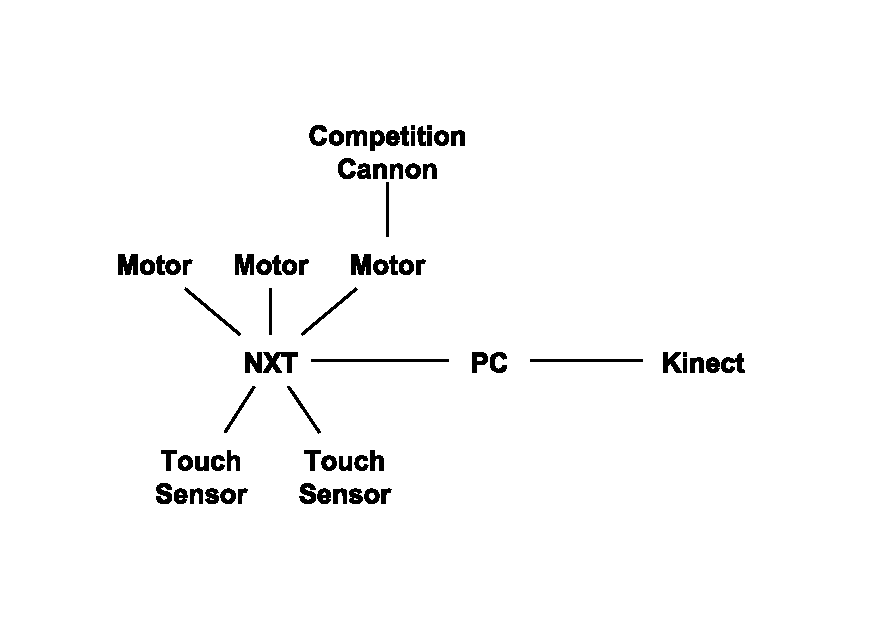
\includegraphics[width=1\textwidth]{img/architecture1.pdf}
\caption{Architecture Diagram} 
\label{fig:archictecture1} 
\end{figure}

\subsection{Software Choices}

\subsubsection*{Operating Systems}
nxtOSEK was chosen for the NXT, because the ability to program in C or C++ gives a lot of control over the
system, and both languages are compiled from source to machine code in a reasonably predictable fashion, which
is one of the main priorities of the system. The various options for scheduling,
while very nice for customizability, did not have much influence on this choice, as the system is simple enough
that it should be doable with most scheduling policies.

For the PC, a Linux operating system was chosen, specifically an Xubuntu 12.04. Linux was chosen for the ease
of installing third party drivers and libraries, and for the slight performance gain over a Windows installation.
Should it prove too slow or unpredictable, it will be easy to move to a Linux server distribution for even
greater performance gains. 

\subsubsection*{Libraries and Languages}
The choice of language for programming the NXT ended up being C, mainly because the primary gain from using C++ was
determined to be object representations of different hardware components. This was considered unnecessary.

Using a Linux PC removes the possibility to use the Microsoft Kinect SDK for communication with the
Kinect camera, so the freenect library will be used instead. And since the targets will be found using image
data, \ac{opencv} will be implemented as well.

The language chosen for implementing the image analysis was Python. Using a high-level scripting language for
this part after arguing for performance and predictability may seem strange, but there are several reasons for
this.

For one, the PC-Kinect part of the system is, from a real-time perspective considered to be a sensor that
happens to be plugged in to the USB port of the NXT, so when it comes to predictability, the important thing is
the data being sent.
When it comes to performance, the Python script itself does not do a lot of calculations, as all libraries used
are implemented as calls to compiled C code. This, combined with the fact that most of the delays in this part
of the system comes from I/O (Kinect and USB), made the group prioritize the ease of writing Python over the
speed of C.
